%!TEX root = ../../thesis.tex


\subsection{Fundamental photon noise limitation}
\label{subsec:fundamental_precision}
A technique to calculate the theoretical radial velocity precision of a spectrum using the full spectral information in an optimal way was first presented by~\citet{connes_absolute_1985}.
Here the radial velocity precision derivation following~\citet{connes_absolute_1985, bouchy_fundamental_2001, figueira_radial_2016} is provided.

\begin{figure}
    \centering
    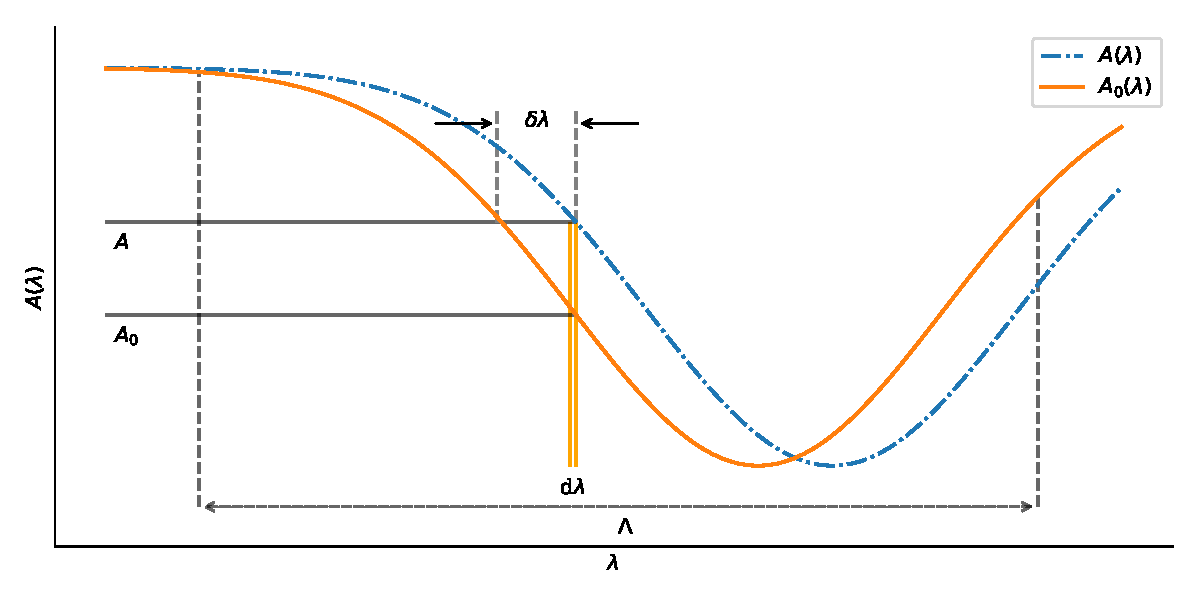
\includegraphics[width=0.8\linewidth]{figures/information-content/precision_plot.pdf}
    \caption[Demonstration of a shifted arbitrary spectral line.]{Arbitrary spectral line with a shift \(\delta \lambda\), inspired by~\citet{connes_absolute_1985}.
        \(\Lambda\) is the wavelength range considered.}
    \label{fig:precisionderivation}
\end{figure}
\todo{add \(\delta A\) to plots}

For demonstration purposes \cref{fig:precisionderivation} shows a portion of an arbitrary spectrum \(A(\lambda)\), over a wavelength range \(\Lambda\).
Here \({A}_{0}(\lambda)\) is the reference spectrum while \(A(\lambda)\) is observed some later time with an apparent wavelength shift observed.
The majority of a single Gaussian line is shown as spectral lines contain the most information but the presence of spectral lines is not a requirement for the derivation.

The Doppler shift of a spectrum is given by:
\begin{equation}
\frac{\delta V}{c} = \frac{\delta \lambda}{\lambda},
\label{eqn:dopplershift}
\end{equation}
where \(c\) is the speed of light in a vacuum, and \(\delta \lambda\) is the shift in wavelength \(\lambda\) due to the velocity \(\delta V\).

\todo{intensity change from connes is vertically in the slice d lambda}

Using basic calculus \(\delta y = \pd{y}{x} \delta x \nonumber\), and for a Doppler shift that is small compared to the line-width\footnote{Although~\citet{connes_absolute_1985} show that the approximation in \cref{eqn:intensitychange} is adequate under all circumstances.}, the observable intensity change in a wavelength slice \(d \lambda\) (or at a given pixel) can be expressed by:
\begin{equation}
\delta A(i) = A(i) - {A}_{0}(i) \simeq \pd{{A}_{0}(i)}{\lambda(i)} \delta \lambda = \pd{{A}_{0}(i)}{\lambda(i)} \frac{\delta V(i)}{c}\lambda(i).
\label{eqn:intensitychange}
\end{equation}

Rearranging \cref{eqn:intensitychange} for \(\delta \lambda\) and combining it with \cref{eqn:dopplershift}, the Doppler shift then becomes:
\begin{equation}
\frac{\delta V(i)}{c} = \frac{A(i) - {A}_{0}(i) }{\lambda(i) (\partial {A}_{0}(i)/\partial \lambda(i))} \label{eqn:delta_v_i}
\end{equation}

This equation shows that the radial velocity measured at pixel {\(i\)}, through a change in the intensity in the recorded spectrum, \(A(i)-{A}_{0}(i)\), and inversely proportional to the slope of the spectrum, \({\partial {A}_{0}(i)}/{\partial \lambda(i)}\).
\Cref{eqn:delta_v_i} provides a separate measurement of the radial velocity shift for every pixel, \(i\), in the spectrum.
The sensitivity of the velocity measurement can be improved, and the noise decreased by using the information from the whole spectral range, \(\Lambda\).
This is achieved by taking the weighted average\footnote{Weighted average on x is \(\bar{x} = \frac{\sum{ x(i)W(i)}}{\sum {W(i)}}\)} over all pixels in the spectral range using an optimal pixel weight \(W(i)\).

\begin{equation}
\overline{\frac{\delta V}{c}} = \frac{\sum{\frac{\delta V(i)}{c}W(i)}}{\sum {W(i)}}.
\end{equation}

Statistically, the optimal weights are proportional to the inverse square of the individual dispersion (variance),
\begin{equation}
W(i) = \frac{1}{{\left(\frac{\delta V_{\rms}(i)}{c}\right)}^{2}}, \label{eqn:weights}
\end{equation}
where \(X_{\rms}\) is the dispersion on the quantity \(X\).

The individual dispersion of the velocity measurement \(\delta V_{\rms}(i)\) is the dispersion that would result from several measurements of the reference spectrum all with the same Doppler shift (e.g.\ zero).
\Cref{eqn:delta_v_i} thus becomes:
\begin{equation}
\frac{\delta V_{\rms}(i)}{c} = \frac{{[A(i) - {A}_{0}(i)]}_{\rms} }{\lambda(i) (\partial {A}_{0}(i)/\partial \lambda(i))}.
\label{eqn:delta_v_i_rms}
\end{equation}
The noise of the spectrum \(A\) is the quadratic sum of the photon noise \(\sqrt{A}\) and the detector noise \({\sigma}_{D}\).
The spectrum \({A}_{0}\) is considered noise free.

\begin{equation}
{[{A(i)-{A}_{0}(i)}]}_{\rms} = {[{A(i)} - 0]}_{\rms} = \sqrt{{\sqrt{A(i)}}^{2} + {{\sigma}^{2}}_{D}} \label{eqn:noise}
\end{equation}

Considering that the Doppler shift is small and that \(A\) and \({A}_{0}\) have the same intensity level, then \(A = {A}_{0}\) can be set.
Using \cref{eqn:delta_v_i,eqn:weights,eqn:noise} the optimum weights then become solely dependent on the reference spectrum.

\begin{equation}
W(i) = \frac{{\lambda}^{2}(i) {({\partial {A}_{0}(i)}/{\partial \lambda(i)})}^{2}}{A_0(i) + {\sigma}^{2}_{D}} \label{eqn:optimal_weight}
\end{equation}

This weighting function can be modified to mask out and eliminate unwanted lines in the spectrum (see \cref{subsec:masking_function}).
For instance setting the particular pixel weights to zero to remove any telluric absorption lines in the observed spectra.

With the optimal weights set, the weighed average velocity change measured from the full spectral range \(\Lambda\), is given by:

\begin{align}
\frac{\overline{\delta V}}{c} &= \frac{
    \sum{
        \frac
        {A(i) - {A}_{0}(i)}{
            \lambda(i) \left({\partial {A}_{0}(i)}/{\partial \lambda(i)}\right)} W(i)}
}
{\sum{{W(i)}}} \\
&= \frac{
    \sum {
        \frac
        {A(i) - {A}_{0}(i)}
        {\lambda(i) (\partial {A}_{0}(i)/\partial \lambda(i))}
        \frac
        {{\lambda}^{2}(i) {({\partial {A}_{0}(i)}/{\partial \lambda(i)})}^{2}}
        {A_{0}(i) + {\sigma}^{2}_{D}}
    }
}
{\sum{{W(i)}}} \\
&= \frac{
    \sum { 
        (A(i) - {A}_{0}(i))
        \frac
        {\lambda(i) {\partial {A}_{0}(i)}/{\partial \lambda(i)}}
        {A_{0}(i) + {\sigma}^{2}_{D}}
    }
}
{\sum{{W(i)}}} \\
&= \frac{\sum{(A(i) - {A}_{0}(i)){\left(\frac{W(i)}{{A}_{0}(i) +{\sigma}_{D}^{2}}\right)}^{1/2}}}{\sum{W(i)}}
\label{eqn:delta_v_eqarray}
\end{align}

The important quantity for {RV} measurements is not just the velocity values themselves but also the dispersion (or uncertainty) on the measured velocity, the {RV} precision \(\delta V_{\rms}\), from the spectrum.
This allows one to assess the planetary detectability limitations attainable in the spectra.
From rearranging \cref{eqn:weights} the dispersion is given by:
\begin{equation}
\overline{\frac{\delta V_{\rms}}{c}} = \frac{1}{\sqrt{\sum{\,W(i)}}} = \frac{1}{Q \sqrt{\sum{\,{A}_{0}(i)}}}.\label{eqn:dv_rms}
\end{equation}
With \cref{eqn:dv_rms} the velocity precision is inversely proportional to the sum of the optimal pixel weights.\todo{An aspect that is quite important and that I think should be stressed out is that this calculation was made for very small line shifts, i.e.\ RV variations, and by this one means much smaller than the line width. For larger ones, the principles here break down.}
Here \(Q\) is a spectral quality factor, defined for the pure photon noise case in~\citet{connes_absolute_1985, connes_demonstration_1996}, as:
\begin{equation}
Q \equiv \frac{\sqrt{\sum{\,W(i)}}}{\sqrt{\sum{\,{A}_{0}(i)}}} = \frac{\sqrt{\sum{\,\frac{{\lambda}^{2}(i) {({\partial {A}_{0}(i)}/{\partial \lambda(i)})}^{2}}{A_0(i) + {\sigma}^{2}_{D}}}}}{\sqrt{\sum{\,{A}_{0}(i)}}}. \label{eqn:quality_factor}
\end{equation}

The pure photon noise case is exclusively considered here in a high signal-to-noise regime in which \({A(i) + \sigma_{D}^{2}} \sim {A(i)}\) can be approximated.
The quality factor, \(Q\), becomes flux independent and is purely a function of the spectral profile within the spectral range considered\footnote{In the case of pure detector noise case the fluctuations in \(A\) are independent of the spectrum \(A\) and the quality factor is \({Q}_{D} = \frac{\sqrt{\sum{{\lambda}^{2} {(\partial {A}_{0}(i)/\partial \lambda(i))}^{2}}}}{\sum{\, {A}_{0}(i)}}\) as derived by~\citet{connes_absolute_1985}.}.
It is a measure of the line richness i.e.\ that quantity and depth of the lines.
For example a spectrum with many sharp lines will have a high \(Q\).
The instrumental resolution of the spectrograph also effects the spectral quality as it induces line broadening.

The radial velocity precision or uncertainty can be rearranged in terms of the spectral quality;
\begin{equation}
\delta V_{\rms} = \frac{c}{Q \sqrt{\sum {\,{A}_{0}(i)}}} = \frac{c}{Q \sqrt{{N}_{{e}^{-}}}} \approx \frac{c}{Q \cdot \snr{}},  \label{eqn:snr_relation}
\end{equation}
where \(\sum {A}_{0}(i) = {N}_{{e}^{-}}\) is considered to be the total number of photo-electrons \({N}_{{e}^{-}}\) counted in the spectral range considered, and \(\snr{}=\sqrt{N_{{e}^{-}}}\) for large \(N_{{e}^{-}}\).

The number of photo-electrons counted \(N_{{e}^{-}}\) in an observed spectrum depends on many factors, such as: the stellar magnitude, detector efficiency and integration time.
It can be estimated using
\begin{equation}
N_{{e}^{-}} = P_{avg} * S_{tel} * \texp * \alpha* \Lambda, \label{eqn:Ne}
\end{equation}
where \(P_{avg}\) is the average monochromatic stellar brightness
across the wavelength range \(\Lambda\) in {\si{\photons\per\second\per\centi\metre\squared\per\centi\metre}},\todo{check}
\(S_{tel}\) is the telescope collecting area in \si{\centi\metre\squared},
\(\texp\) is the integration time in \si{\second}, and \(\alpha\) the is overall system efficiency (including atmosphere, telescope, spectrograph and detector).

This technique has been tested and demonstrated on observations by~\citet{connes_demonstration_1996} and been used to predict the accuracy or performance limits of new spectrograph instrumentation~\citep[e.g.][]{connes_absolute_1985,butler_attaining_1996,bouchy_fundamental_2001} and has informed the design (and use) of spectrographs, e.g.\ {SPIRou}~\citep{artigau_spirou_2014,figueira_radial_2016}.
However,~\citet{figueira_radial_2016} bypass the calculation of \(N_{{e}^{-}}\) in \cref{eqn:Ne} by scaling the synthetic spectral models to a specific \snr{} level instead.

In the case of several \(\delta V\) measurements computed for \(k\) spectral slices (or spectral orders) then the error on the average \(\overline{\delta V}\) is given by the error on a weighted average:
\begin{equation}
\overline{\delta {V}_{\rms}} = \frac{1}{\sqrt{\sum_k{{(\frac{1}{\delta V_{\rms}(k)})}^{2}}}}. \label{eqn:weighted_average_error}
\end{equation}

A separate general formula for {RV} precision, discussed in \cref{sec:rv_precision}, is given by~\citet{hatzes_spectrograph_1992} in terms of general spectral parameters:
\begin{equation}
\delta V_{\rms} = \frac{1}{\sqrt{F} \sqrt{\Lambda} {R}^{1.5}}
\end{equation}
where $\sqrt{F}$ represents the \snr{} of the spectrum in the {Poisson}-noise dominated regime, and \(R\) is the spectral resolution.
The $\Lambda$ comes from assuming a homogeneous distribution of lines, with the same line properties, per unit length.

